\begin{Exercise}[label = boatgraph, origin = {Jaan Kalda, \url{http://www.ioc.ee/~kalda/ipho/}}, difficulty = 3, title = Bootsbewegung]
	Die Beschleunigung eines Boots hängt von seiner Geschwindigkeit ab, wie im Bild gezeigt. Die Anfangsgeschwindigkeit des Bootes beträgt $v_0 = 4~\nicefrac{m}{s}$. Wie groß ist die Strecke, die das Boot zurücklegt hat, wenn es nahezu zum stehen kommt?
\end{Exercise}
\begin{figure}[h]
	\centering
	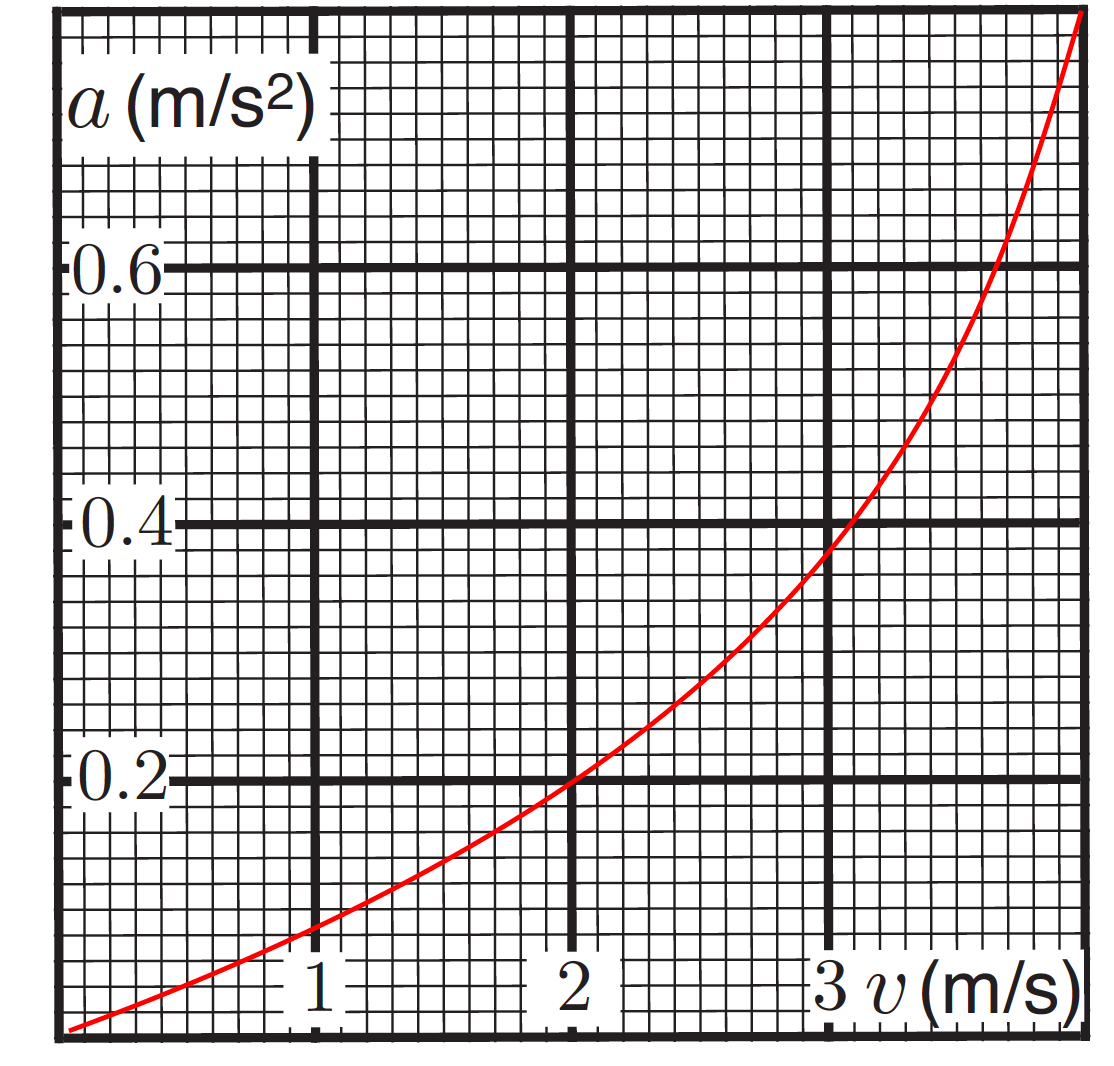
\includegraphics[scale = 0.4]{../tasks/kalda/boatgraph1}
\end{figure}
\begin{Answer}[ref=boatgraph]
	Die insgesamt zurückgelegte Strecke ist das Integral der Geschwindigkeitsfunktion
	\begin{equation}\label{boatgraph:sdef}
		v = \frac{ds}{dt}\Rightarrow s = \int_{0}^{\infty}ds = \int_{0}^{\infty} v~dt.
	\end{equation}
	Nun haben wir aber die Geschwindigkeit $v$ nicht als Funktion der Zeit gegeben. Deswegen müssen wir mit den Differentialen tricksen.\\
	Da wir die Beschleunigung als Funktion der Geschwindigkeit gegeben haben, ist das ein guter Anhaltspunkt. Es gilt nämlich
	\begin{equation}\label{boatgraph:adef}
		a  = \frac{dv}{dt} \Rightarrow dt = \frac{1}{a} dv.
	\end{equation}
	Das können wir jetzt in \eqref{boatgraph:sdef} einsetzten, und kommen auf
	\begin{equation}
		s = \int_{0}^{\infty} \frac{v}{a}~dv.
	\end{equation}
	Das heißt, wir müssen einfach $\frac{v}{a}$ als Funktion von $v$ abtragen, und den gesamten Flächeninhalt unter der Funktion bestimmen. Das dauert eine Weile. Am Ende kommt $s\approx 72~\mathrm{m}$ raus.
\end{Answer}